\documentclass{article}
\usepackage[T1]{fontenc}
\usepackage{lmodern}
\usepackage{graphicx}
\usepackage{amsmath,amssymb}
\usepackage[a4paper,margin=2cm]{geometry}
\usepackage[absolute,overlay]{textpos}
\setlength{\TPHorizModule}{1mm}
\setlength{\TPVertModule}{1mm}
\usepackage[indonesian]{babel}
\usepackage{hyperref}
\setlength{\emergencystretch}{2em}
% unit: Halaman 50

\begin{document}

% === Halaman 50 (llm) ===

\section*{Triple DES (TDES)}

\vspace{71.28mm}

\begin{itemize}
    \item Menggunakan DES tiga kali
    \item Bertujuan untuk mencegah \textit{meet-in-the-middle attack}.
    \item Bentuk umum Triple DES (mode EEE):
    \begin{align*}
        \text{Enkripsi: } C &= E_{K3}(E_{K2}(E_{K1}(P)))\\ 
        \text{Dekripsi: } P &= D_{K1}(D_{K2}(D_{K3}(C)))
    \end{align*}
\end{itemize}

\vspace{20mm}

% deskripsi: Diagram blok proses enkripsi Triple DES (EEE) dengan tiga tahap enkripsi (E) menggunakan kunci K1, K2, dan K3 secara berurutan.
% bbox normalisasi: [0.5120, 0.3970, 0.9900, 0.6370]
\begin{textblock*}{100.38mm}(107.52mm,117.91mm)
\noindent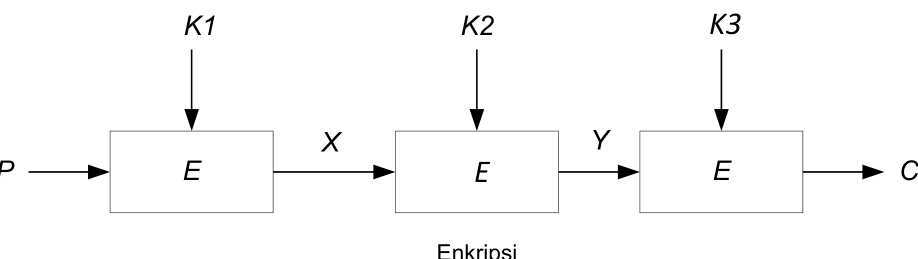
\includegraphics[width=100.38mm,height=71.28mm]{../../images/llm/page_050_img_01.png}%
\end{textblock*}

% deskripsi: Diagram blok proses dekripsi Triple DES (EEE) dengan tiga tahap dekripsi (D) menggunakan kunci K3, K2, dan K1 secara berurutan.
% bbox normalisasi: [0.5120, 0.6950, 0.9900, 0.9350]
\begin{textblock*}{100.38mm}(107.52mm,206.41mm)
\noindent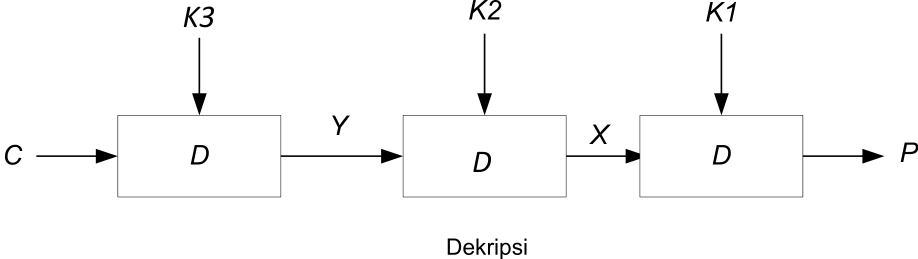
\includegraphics[width=100.38mm,height=71.28mm]{../../images/llm/page_050_img_02.png}%
\end{textblock*}

\end{document}
